\documentclass[UTF8,10pt,a4paper]{ctexart}
\usepackage[utf8]{inputenc}
\usepackage{amsmath}
\usepackage{amsfonts}
\usepackage{amssymb}
\usepackage{graphicx}

\author{陈斯杰}
\title{Chapter1. THE GENESIS OF FOURIER ANALYSIS}
\begin{document}
\maketitle
\begin{abstract}
This book begins the talk of Fourier Analysis with two 
physical problem: vibrating string and heat conduction.
In this review, I am going to illustrate these two examples
in detail by supplementing the background knowledge.
\end{abstract}

\section{The Vibrating String}
	\subsection{Simple harmonic motion 简谐运动}
		\begin{figure}[ht]
			\centering
			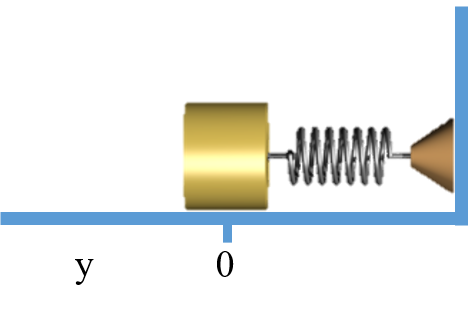
\includegraphics[width=5cm]{idealspring.png}
			\caption{简谐运动谐振子}
			\label{fig:xiantu}
		\end{figure}
		
		\noindent		
		Newton's law produces a 2nd order ODE

		\begin{equation}
			F=-ky(t) \Rightarrow -ky(t)=my''(t)
		\end{equation}

		Let $c=\sqrt{\frac{k}{m}}$, we get a neater form: 
		
		\begin{equation}
			y''(t)+c^2y(t)=0
		\end{equation}				
		
		Equation(2)	is a linear homogeneous 2nd-order differential equation(二阶常系数线性方程).
		For a general case $y''+py'+qy=0$, we first solve the characteristic equation
		$\lambda^2+p\lambda+q=0$ and get the characteristic roots: $\lambda_1, \lambda_2$.
		
		\begin{tabular}{|lll|}
		\hline
		Characteristic Roots & Linear Independent Sol. Pair & General Sol.\\
		\hline
		$\lambda_1,\lambda_2\in\mathbb{R}\ and\ \lambda_1\neq\lambda_2$ &
		$y_1=e^{\lambda_1 x}, y_2=e^{\lambda_2 x}$ &
		$y=C_1e^{\lambda_1 x}+C_2e^{\lambda_2 x}$ \\
		
		$\lambda_1,\lambda_2\in\mathbb{R}\ and\ \lambda_1=\lambda_2$ &
		$y_1=e^{\lambda_1 x}, y_2=xe^{\lambda_1 x}$ &
		$y=(C_1+C_2x)e^{\lambda_1 x}$ \\
		
		$\lambda_1,\lambda_2=\alpha\pm i\beta$ &
		$y_1=e^{\alpha x}cos\beta x, y_2=e^{\alpha x}sin\beta x$ &
		$y=e^{\alpha x}(C_1 cos\beta x +C_2 sin\beta x)$ \\
		\hline
		\end{tabular}
\end{document}